\documentclass[10pt, conference]{FMFP2022}
\usepackage[top=1.50cm, bottom=1.50cm, left=1.884cm, right=1.884cm, includehead, includefoot, heightrounded]{geometry}
\usepackage{fancyhdr} % To use headers
\usepackage{graphicx} %To use graphics package
\usepackage[textfont=bf, font = normalsize]{caption} %To use bold and normal size font for table and figure captions
\usepackage{floatrow} %To have table captions above the table
\usepackage{amssymb}
\usepackage{amsfonts}
\usepackage{amsmath}
\floatstyle{plaintop} %To have table captions above the table
\restylefloat{table} %To have table captions above the table
\usepackage{subfigure} % To use subfigures
 \floatsetup{font = normalsize} %Size of font in tables
    
\rhead{
	\sffamily\fontsize{9}{11}\selectfont
	\vspace{-0.5cm}
	\textbf{Proceedings of the 9th International and 49th National Conference on Fluid Mechanics and Fluid Power (FMFP) \\ December 14-16, 2022, IIT Roorkee, Roorkee-247667, Uttarakhand, India} \\ \vspace{0.15cm}
	\large{\textbf{FMFP2022-XX-YYY}}}

\renewcommand{\headrulewidth}{0pt}


\begin{document}

\title{\LARGE{ \bf The Title of a Sample Paper for FMFP 2022 prepared using LaTex}}
\author{\textbf{Krishna M. Singh\textsuperscript{1}, M. R. Ravi\textsuperscript{1}, Toshiro Matsumoto\textsuperscript{2}, and Sudhakar Subudhi\textsuperscript{3}}\\\\
\textsuperscript{1}\small{Department of Mechanical and Industrial Engineering, IIT Roorkee, Roorkee-247667, India}\\
\textsuperscript{2} \small{Department of Mechanical Engineering, IIT Delhi, New Delhi-110016, India}\\
\textsuperscript{3} \small{Department of Mechanical Science and Engineering, Nagoya University, Nagoya, Japan}}

\maketitle
\thispagestyle{fancy} 
\pagestyle{plain} % To suppress headers but still include page numbers from second page on

\noindent \textbf{ABSTRACT}

The abstract should be limited to 150-200 words. We present direct numerical simulations of the statistical properties of the thermal dissipation rates in the turbulent Rayleigh-B\'{e}nard convection for the fluid of $Pr=0.7$ contained in a cubic cell. The Rayleigh numbers $Ra$ is varied between $10^6$ and $2\times10^8$. Based upon the criterion whether the product of the vertical velocity and the temperature fluctuation ($w\theta$) is positive or negative we decompose the whole cell volume into plume dominated and the background dominated regions.
\\\\
\noindent
\textbf{Keywords:} Insert 3-4 keywords that categorize the work\\

\section{{\textbf{INTRODUCTION}}}
Thermal convection has been of major interest to the scientific community owing to its ubiquitous presence in many natural flows, such as, earth's core, Sun, Ocean, atmosphere, and their applications in many science and engineering problem wherever heat convection plays important role. Thermal convection is one of the few systems in which system approaches to the turbulent state upon increase in the parameter quite systematically, i.e., static region is followed by the time dependent region and then chaos which is followed by the spatio-temporal chaos and then the turbulence \cite{Gsell2017}. Among convective systems, Rayleigh-B\'{e}nard convection (RBC) is an ideal model in which a thin layer of the fluid is heated from the bottom and cooled from the top. 

A recurring theme in both theoretical descriptions and phenomenological pictures of RBC is how the heat gets transported from the hot bottom plate to the top cold plate, what are roles of the thermal plumes in the heat transport and the dissipation rates. In this paper we focus on the statistics of the heat transport and the thermal dissipation rates. The thermal dissipation rate is defined as $\epsilon_T(\mathbf{x},t)=\kappa|\nabla T|^2$, which is a measure of the gradient in the turbulent temperature fluctuations. We decompose the contributions to the heat dissipation rates into two parts: due to the thermal plumes and due to the background and numerically analyze their variations with the Rayleigh numbers. Planar modulation of the uniform flow promotes strong asymmetry in the ensuing wake which is otherwise symmetric in time average sense. In one of the first experimental study, delay in onset of vortex shedding due to the presence of planar shear was found. We have not performed the detailed statistical studies of the probability distribution function of the background thermal dissipation rates and the thermal plumes dissipation rates. The studies are under investigation.
 
\section{\textbf{METHODOLOGY}}\label{sec2}
For incompressible, buoyancy driven flow, the normalized governing equations (using the Boussinesq approximation) are
\begin{eqnarray}
R[\dot{G}(z, t)]=\dot{F}[\dot{G}(z, t)]+\Phi[\dot{G}]
\end{eqnarray}
where, $x_i (i=1,2, 3)$ represent the spatial coordinates ($x,y,z$) with $y$ being the vertical direction, $u_i(u, v,w)$ are the velocity components, $p$ the pressure and  $\theta$ the normalized temperature ($\theta=(T-T_C)/(T_H-T_C)$) with $T$ is the instantaneous temperature and $T_H$, $T_C$ are, respectively, the temperature of the hot and cold plates. We have used  $H,~\sqrt{g \alpha \Delta T H}$ and $~(T_H-T_C)$  as the scales for normalization of length, velocity and temperature, respectively. Equations \ref{eq1}-\ref{eq3} are discretized using finite volume framework. The same could be written as finite volume framework is used to discretize Eqs. \ref{eq1}-\ref{eq3}. No-slip condition is implemented for all the velocity components on the walls, while for temperature, isothermal condition is applied on the horizontal walls and no-flux (adiabatic) conditions is applied on the vertical walls. Hence, at the top and bottom solid walls, the temperature takes specified values (0 and 1).

\subsection{\textbf{Validation}}\label{sec2p1}
The simulation details are given in the Table~\ref{table2}. To validate our code we computed the Nusselt numbers through three different ways \cite{Panton2009}: (a) using the mean heat flux at the horizontal surfaces near the hot and bottom plates ($Nu_S$), (b) using the heat dissipation ($Nu_{\epsilon_T}={(RaPr)}^{1/2}<\epsilon_T>_{global}$), and (c) using the viscous dissipation ($Nu_{\epsilon_u}={(RaPr)}^{1/2}<\epsilon_u>_{global}+1$).

\begin{figure}
\centering
\includegraphics[width=0.8\textwidth]{figure1.eps}
\caption{Variations of the percentage volume occupied by the plume and the background in the cubic cell with $Ra$ for different threshold value $\delta$.}
\label{figure1}
\end{figure} 

\section{\textbf{RESULTS AND DISCUSSION}}\label{sec3}
All the figures and Tables should be referred in order of their appearances. Figure \ref{figure1} should be written if it appears at the start of a sentence, while Fig. \ref{figure1} is the correct way otherwise. However, Table \ref{table2} should appear in full irrespective of its position. In RBC one of the central theme of the turbulent research is to get the scalings for the dissipation rates and further establish its connection with the nature of heat transport in the turbulent state \cite{Pascal2000}. A plume can be defined in the region where there is strong correlation between the vertical velocity ($w$) and the temperature fluctuations defined as  $\theta(\textbf{x},t)=T(\textbf{x},t)-\langle T(z)\rangle_{A,t}$ where, $<.>_{A,t}$ is the averaged over horizontal plane and the time, exists. 

\begin{table}
\centering
\caption{The values of the fitting parameters}%\vspace{-10pt}
\begin{tabular}{|c|c|c|c|c|}
\hline
$\delta(\%)$   & $A_{pl}$ & $\beta_{pl}$& $A_{bg}$ &$\beta_{bg}$  \\ 
\hline
 $0$&$0.138$  &$-0.197$ &$0.553$ & $-0.269$\\
$0.1$&$0.115$  &$-0.198$ &$0.838$ &$-0.279$ \\
$1$&$0.072$  &$-0.182$ &$0.919$ &$-0.287$ \\
$5$&$0.033$  &$-0.144$ &$0.531$ &$-0.265$\\
$10$&$0.02$  &$-0.118$ &$0.377$ &$-0.248$\\
\hline
\end{tabular}
\label{table2}
\end{table}

\begin{figure}
\centering
\includegraphics[width=0.8\textwidth]{figure2.eps}
\caption{Variations of the contribution of the plumes and the background to the heat dissipation rates with the Rayleigh number.}
\label{fig:3}
\end{figure} 
All the references that appear in the section ``REFERENCES" should be cited appropriately in the text. In Fig.~\ref{figure1} we show the variation of the volume fraction of the plume and background with the Rayleigh numbers for different threshold value ($\delta$), where, $<\epsilon>_{V_{pl},t}$ and $<\epsilon>_{V_{bg},t}$ are respectively the contributions from the plume and background into the thermal dissipation rates. Figure \ref{fig:3} shows the variation of the thermal dissipation rate with the Rayleigh number along with the separate contribution from the plume ($\epsilon{pl}$) and background ($\epsilon_{bg}$) to the thermal dissipation rates for the threshold $\delta=0$. We find that the contribution from the plume and background to the thermal dissipation rates approaches to nearly equal for the highest Rayleigh number ($Ra\sim 10^8$).

\section{\textbf{CONCLUSIONS}}\label{sec4}
In the paper we have presented the statistics of the energy dissipations rate. Based upon the criterion the cell region is locally identified as the plume dominated region or the background depending on whether the product of the vertical velocity and the temperature fluctuation  ($w\theta$) is greater or less than the threshold value ($\delta$).  We have considered different values of the $\delta$. For all the threshold $\delta$ the volume fraction of the plume as well as background exhibit the power law behavior. The exponent is in good agreement of the earlier reported numerical simulation. Further we have computed the dependence of the contribution of the plumes and backgrounds to the thermal dissipation rates and found that both contribution exhibits decreasing trend with the Rayleigh number. Both the contributions become equal at high $Ra$. 

\vspace{0.5cm}
\noindent
\textbf{ACKNOWLEDGEMENTS}\\
\noindent If the authors want to acknowledge any person, institute, or facilities, it may be done here. \\

\vspace{0.5cm}
 \noindent
\textbf{NOMENCLATURE}\\

\begin{tabular}{ccc}
$A$ & Frontal area of rotor & [m$^2$]\\
$Re$ & Reynolds number & -- \\
$\epsilon$ & Dissipation & --
\end{tabular}

\bibliographystyle{amsplain}
\bibliography{FMFP2022}

    
\end{document}
